\documentclass{LabReport}
\title{操作系统实验报告PA7}
\author{221900180 田永铭}
\date{\today}
\addbibresource{refs.bib}
\Chead{操作系统实验报告PA7 221900180 田永铭}
\Cfoot{\thepage}
\usepackage{listings}
\usepackage{graphicx} 
\usepackage{tikzsymbols}
\usepackage{tikz}
\usepackage{hyperref}

\lstset{
	basicstyle=\ttfamily, % 设置等宽字体
	frame=shadowbox,
	language=C,
	showspaces=false % 不显示空格
	showstringspaces=false % 不显示字符串中的空格
	showtabs=false, % 不显示制表符
}

\begin{document}
	\maketitle
	
	\tableofcontents
	
	\newpage
	
	\section{实验要求}
试根据课堂给出的基于信号量PV操作的读者-写者(读者优先)同步算法实现一个读写锁,并设计一个方案用于测试pthread库中提供的读写锁pthread\_rwlock与前述读写锁,分析其表现是否一致?\par
\hspace{0em}需基于gcc和pthread库实现上述内容,并根据运行结果进行论述。\par
\hspace{0em}提示:\par\hspace{0em}
1)明确读者优先、读写公平的概念;\par\hspace{0em}
2)测试方案可创建若干读、写线程,利用sleep设定读写线程间合理的读、写申请顺序,以及模拟读、写的持续时间。

	\section{实验环境}
	
	\begin{itemize}
		\item 操作系统:wsl2
		\item 编程语言:C语言
		\item 使用工具:gcc编译,pthread库等
		\item 虚拟系统版本:Ubuntu-22.04
	\end{itemize}
	
	\section{实验原理}
	\begin{itemize}
	\item \textbf{PV信号量的原理:}
	
	PV操作是Dijkstra在提出信号量(Semaphore)时引入的两种原子操作,其中P操作表示“测试(Proberen)”或“等待(Wait)”,V操作表示“增加(Verhogen)”或“信号(Signal)”。信号量用于管理对公共资源的访问,其操作原理如下:
	
	\begin{itemize}
		\item \textbf{P操作:}如果信号量的值大于0,将其减1;如果信号量的值为0,进程被阻塞,直到信号量的值大于0。
		\item \textbf{V操作:}将信号量的值加1,如果有被阻塞的进程,则唤醒一个被阻塞的进程。
	\end{itemize}
	
	信号量主要用于实现进程间的同步与互斥,确保多个进程在访问共享资源时不会产生冲突。
	
	\item \textbf{读写锁的原理:}
	
	读写锁是一种同步机制,允许多个线程同时读取共享资源,但在有线程写入共享资源时,必须确保没有其他线程在读取或写入。读写锁的主要原理包括:
	
	\begin{itemize}
		\item \textbf{读者优先:}当一个读者请求访问资源时,如果没有写者在访问资源,则允许该读者访问。多个读者可以同时访问资源。只有当没有读者访问资源时,写者才能获得访问权限。
		\item \textbf{写者优先:}当一个写者请求访问资源时,不再允许新的读者进入,若正在读,那么等到所有当前的读者完成后,写者立即访问资源,而不让新的读者再插队。
		\item \textbf{公平性:}保证读者和写者都能公平地访问资源,不会出现读者或写者长时间等待的情况。
	\end{itemize}
	
	在实现读写锁时,通常使用信号量和计数器来跟踪读者和写者的数量,并通过条件变量或其他同步机制来管理对共享资源的访问。
	
	\end{itemize}
	
	\section{实验过程}
	\par\hspace{0em}实验主要分为以下几个步骤:
	
	\begin{enumerate}
		\item 编写代码框架以及适合本实验的测试样例
		\item 利用pthread标准库提供的读写锁来实现
		\item 自己实现读者优先的读写锁
		\item 自己实现写者优先的读写锁
		\item 自己实现读写公平的读写锁
	\end{enumerate}
	
	\subsection{编写代码框架以及适合本实验的测试样例}
	
	\subsubsection{编写代码框架}
	
	根据老师的提示,我们只需要通过sleep一段时间来模仿读、写的过程,不需要具体的读写内容。所以代码的核心就变为了三个核心部分:读者如何上锁、写者如何上锁以及如何测试锁,以下是读者和写者的相关框架代码,其中rdlock、wrlock、unlock都是一个抽象的、待实现的锁方法。
	
\begin{lstlisting}[language=python,frame=shadowbox]
// 读
void* reader(void* arg) {
	rdlock(&rwlock);
	printf("Pthread Reader %ld is reading...\n", (long)arg);
	sleep(1);
	printf("Pthread Reader %ld finished reading.\n", (long)arg);
	unlock(&rwlock);
	return NULL;
}
\end{lstlisting}

\begin{lstlisting}[language=python,frame=shadowbox]
// 写
void* writer_pthread(void* arg) {
	wrlock(&rwlock);
	printf("Pthread Writer %ld is writing...\n", (long)arg);
	sleep(1);
	printf("Pthread Writer %ld finished writing.\n", (long)arg);
	unlock(&rwlock);
	return NULL;
}
\end{lstlisting}

	这里,我通过printf函数来打印信息,从而方便后续对线程在读还是在写进行测试。而其中的抽象的锁方法正是待实现的部分。
	
\subsubsection{编写适合本实验的测试样例}

要想测试出读写锁是读者优先、写者优先还是读写公平的,需要编写合适的测试样例。最终我的选择是这样的:\\
对于任意的方式,我先后来到的读写线程分别为:读-写-读-写-读-读-读。具体代码如下:
\begin{lstlisting}[language=python,frame=shadowbox]
int main() {
// 测试自定义读写锁
initialize_rwlock();
	
pthread_t readers[5], writers[2];
for (long i = 0; i < 5; i++) {
	pthread_create(&readers[i], NULL, reader, (void*)i);
	sleep(0.0001);
	if (i < 2) {
		pthread_create(&writers[i], NULL, writer, (void*)i);
		sleep(0.0001);
	}
}
	
for (int i = 0; i < 5; i++) {
	pthread_join(readers[i], NULL);
	if (i < 2) {
		pthread_join(writers[i], NULL);
	}
}

destroy_rwlock();
}
\end{lstlisting}

注意:为了并发中防止微小的误差(小到线程运行到哪一行语句),每种方式下我在创完每一个线程后,紧接着就sleep(0.0001),这样能够更严谨的保证读者写着到来的顺序严格地是``读-写-读-写-读-读-读",运行到申请锁的语句的顺序也严格地是``读-写-读-写-读-读-读"。\\
而对于读和写sleep的秒数,我都设置成1秒钟。\\
具体地,这样的设置如何能测验出读写锁的优先方式,我将在实验结果部分展示。

\subsection{利用pthread标准库提供的读写锁来实现}

首先是利用pthread标准库提供的读写锁,这个比较简单,直接调用库即可,核心语句如下:

\begin{lstlisting}[language=python,frame=shadowbox]
// 使用pthread库提供的读写锁定义
pthread_rwlock_t rwlock;
//上读锁
pthread_rwlock_rdlock(&rwlock);
//上写锁
pthread_rwlock_wrlock(&rwlock);
//释放锁
pthread_rwlock_unlock(&rwlock);
//初始化锁
pthread_rwlock_init(&rwlock, NULL);
//销毁锁
pthread_rwlock_destroy(&rwlock);
\end{lstlisting}

将这些语句填入框架,即可实现pthread库提供的读写锁。运行结果我将在实验结果部分展示,在此之前,为了使得实验有更加直观的表现,我分别自己实现一个读者优先、写着优先、读写公平的锁,见以下部分。


\subsection{自己实现读者优先的读写锁}

仅在读者优先的部分展示较全的代码,后面只展示核心部分,读者优先代码如下:
\begin{lstlisting}[language=python,frame=shadowbox]
// 自定义读者优先的读写锁
sem_t rw_mutex;  //读写的锁
sem_t mutex;     //对读者的read_count的锁保护
int read_count = 0;	//读者的数量

void initialize_rwlock() {
	sem_init(&rw_mutex, 0, 1);
	sem_init(&mutex, 0, 1);
}

void reader_lock() {
	sem_wait(&mutex);
	read_count++;
	if (read_count == 1) {
		sem_wait(&rw_mutex);
	}
	sem_post(&mutex);
}

void reader_unlock() {
	sem_wait(&mutex);
	read_count--;
	if (read_count == 0) {
		sem_post(&rw_mutex);
	}
	sem_post(&mutex);
}

void writer_lock() {
	sem_wait(&rw_mutex);
}

void writer_unlock() {
	sem_post(&rw_mutex);
}

void destroy_rwlock() {
	sem_destroy(&rw_mutex);
	sem_destroy(&mutex);
}
\end{lstlisting}

	实现方式比较简单,简单来说就是读者数量只要大于0,那么写者永远无法申请到读写锁。
	
\subsection{自己实现写者优先的读写锁}

	为了实现写者优先的锁,思路是利用一个令牌、或者叫彩票,即``token"变量,读者需要先申请到这个变量,之后才能进行操作。而这个token被第一个写者获得,且由最后一个写者释放。同时,需要额外增加一个变量write\_waiting来统计正在等待或执行的写者数量以及相应的信号量保护它。核心代码如下:
	
	\begin{lstlisting}[language=python,frame=shadowbox]
void reader_lock() {
	sem_wait(&token); // 获取令牌
	sem_wait(&mutex_reader);
	read_count++;
	if (read_count == 1) {
		sem_wait(&rw_mutex);
	}
	sem_post(&mutex_reader);
	sem_post(&token); // 释放令牌
}

void reader_unlock() {
	sem_wait(&mutex_reader);
	read_count--;
	if (read_count == 0) {
		sem_post(&rw_mutex);
	}
	sem_post(&mutex_reader);
}

void writer_lock() {
	sem_wait(&mutex_writer);
	write_waiting++;
	if (write_waiting == 1) {
		sem_wait(&token); // 第一个写者获取令牌
	}
	sem_post(&mutex_writer);
	sem_wait(&rw_mutex);
}

void writer_unlock() {
	sem_post(&rw_mutex);
	sem_wait(&mutex_writer);
	write_waiting--;
	if (write_waiting == 0) {
		sem_post(&token); // 最后一个写者释放令牌
	}
	sem_post(&mutex_writer);
}
	\end{lstlisting}

\subsection{自己实现读写公平的读写锁}

为了实现读写公平的读写锁,思路也是利用一个令牌、或者叫彩票,即``token"变量,只不过这回,读者需要先申请到这个变量,之后才能进行操作,同时写者也需要先申请这个变量,之后才能操作。而这个token被第一个写者获得,且由最后一个写者释放。同时,需要额外增加一个变量write\_waiting来统计正在等待或执行的写者数量以及相应的信号量保护它。核心代码如下:

\begin{lstlisting}[language=python,frame=shadowbox]
void reader_lock() {
	sem_wait(&token); // 获取令牌
	sem_wait(&mutex_reader);
	read_count++;
	if (read_count == 1) {
		sem_wait(&rw_mutex);
	}
	sem_post(&mutex_reader);
	sem_post(&token); // 释放令牌
}

void reader_unlock() {
	sem_wait(&mutex_reader);
	read_count--;
	if (read_count == 0) {
		sem_post(&rw_mutex);
	}
	sem_post(&mutex_reader);
}

void writer_lock() {
	sem_wait(&token); // 获取令牌
	sem_wait(&rw_mutex);
}

void writer_unlock() {
	sem_post(&rw_mutex);
	sem_post(&token); // 释放令牌
}
\end{lstlisting}

	\section{实验结果}
	
	由于我分别写了自己实现的读者优先、写者优先、读写公平的读写锁,所以我先展开论述这三者的表现,再简单地看一看pthread标准库是哪种实现。
	
	\subsection{自己实现的各类锁的表现}
	以下分别是我自己实现的读者优先、写者优先、读写公平的读写锁的表现,测试样例读写申请顺序为``读-写-读-写-读-读-读":\newpage\par
\begin{figure}[h!]
	\centering
	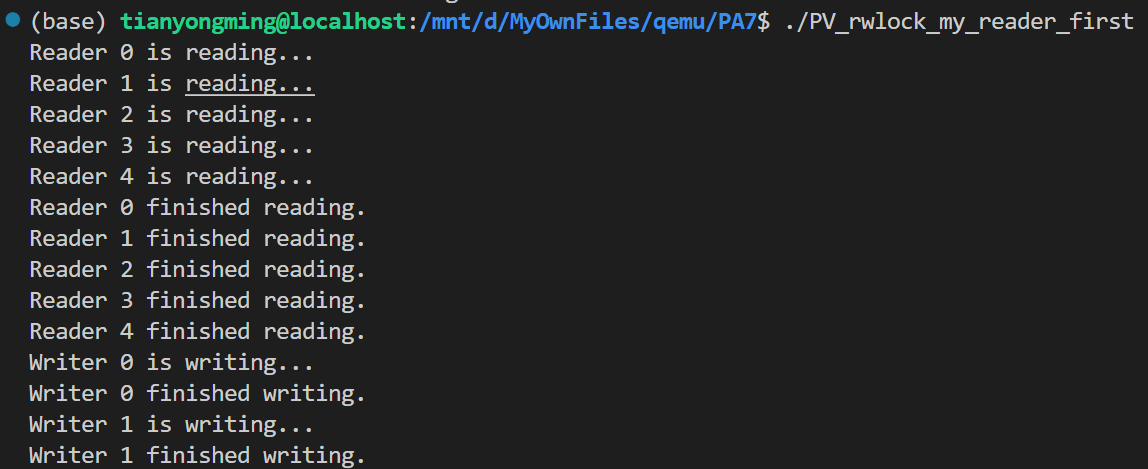
\includegraphics[width=0.85\linewidth]{figures/my_reader_first}
	\caption{读者优先(读-读-读-读-读-写-写)}
	\label{fig:myreaderfirst}
\end{figure}
	
\begin{figure}[h!]
	\centering
	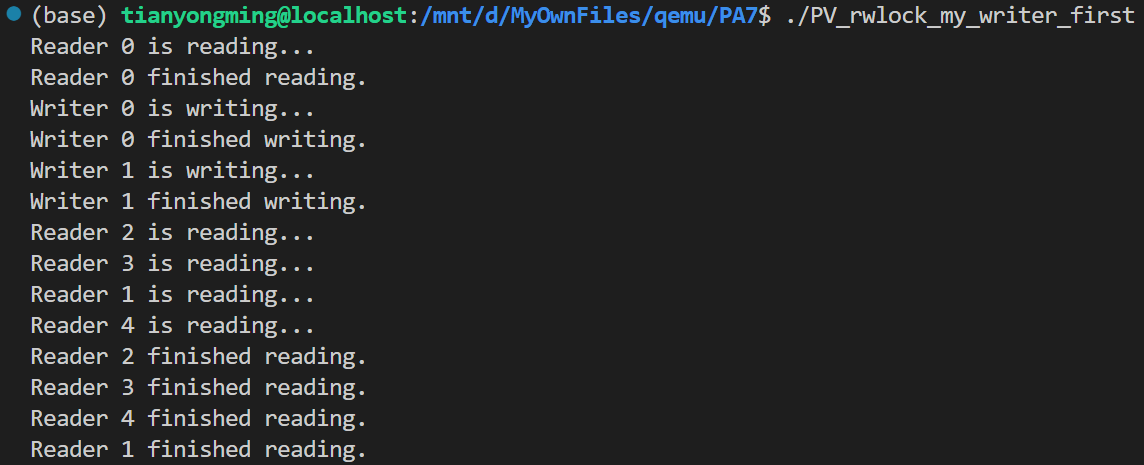
\includegraphics[width=0.85\linewidth]{figures/my_writer_first}
	\caption{写者优先(读-写-写-读-读-读-读)}
	\label{fig:mywriterfirst}
\end{figure}
	
\begin{figure}[h!]
	\centering
	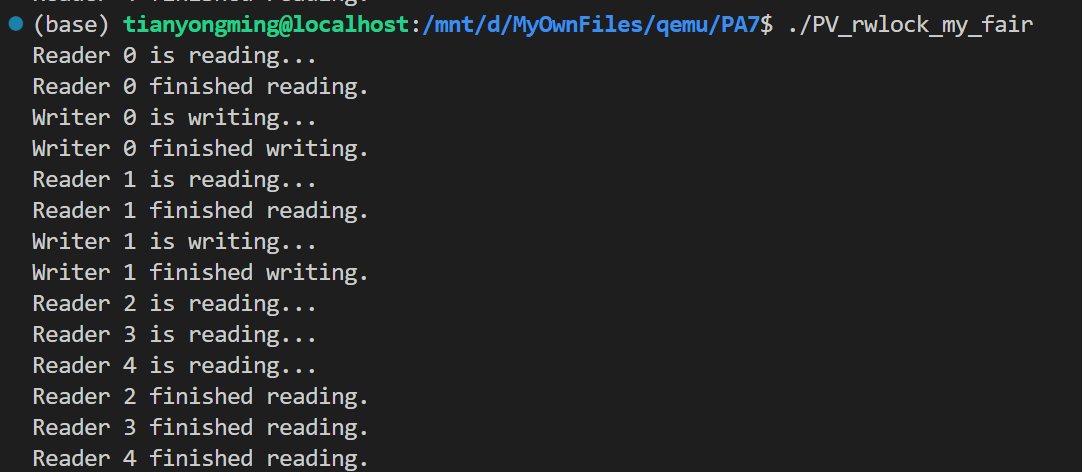
\includegraphics[width=0.85\linewidth]{figures/my_reader_and_writer_fair}
	\caption{读写公平(读-写-读-写-读-读-读)}
	\label{fig:myreaderandwriterfair}
\end{figure}
	
	对比之下,实验结果真的可谓一目了然。接下来对三个实验的结果进行详细解读:
	\begin{enumerate}
		\item \textbf{读者优先的情况下:}由于先申请的读者,后续的写者只有等读者读完才能写,所以直到最后申请的三个读者全部完成后写者才能开始写。所以呈现了如上结果。
		\item \textbf{写者优先的情况下:}由于token令牌只能由第一个写者获得,所以第一个读者读完之后,令牌就落在了写者手里,知道最后一个写者写完,写者数量清零,才释放令牌,此后读者才能再读。所以呈现了如上结果。
		\item \textbf{读写公平的情况下:}由于读者写者操作前都需要申请token令牌,那么在这样的公平的形式下,基本是按照申请顺序来进行操作的,即先来先到。所以呈现了如上结果。
	\end{enumerate}
	
	\subsection{pthread标准库读写锁的实现}
	以下是pthread库pthread\_rwlock\_t对读写锁的实现,测试样例读写申请顺序为``读-写-读-写-读-读-读":
	
\begin{figure}[h!]
	\centering
	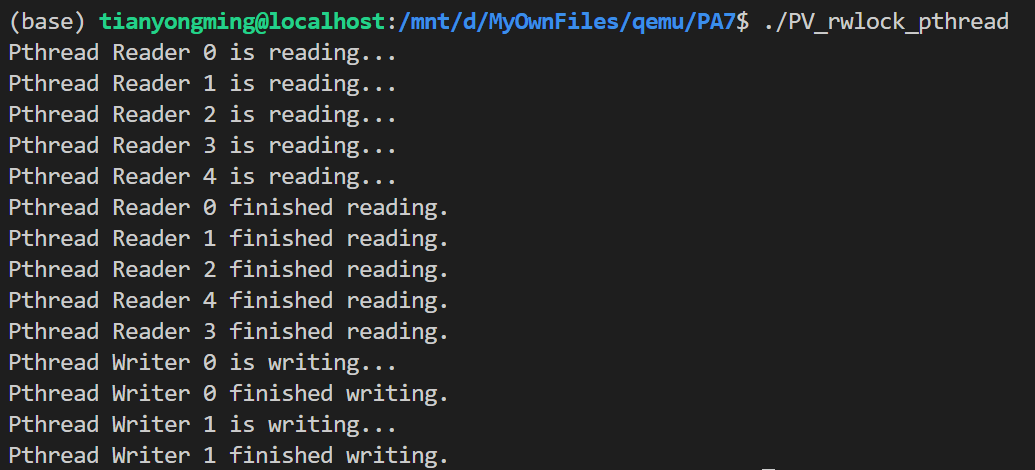
\includegraphics[width=0.9\linewidth]{figures/pthread}
	\caption{pthread读写锁(读-读-读-读-读-写-写)}
	\label{fig:pthread}
\end{figure}

	显示,标准库是用的读者优先的方式实现的读写锁。

	\section{拓展分析}
	更掘一隅,为什么pthread标准库是利用读者优先的方式来实现读写锁的呢?是不是不能有其它方式实现?
	
	\subsection{为什么pthread标准库是利用读者优先的方式来实现读写锁}
	选择读者优先策略来实现读写锁有以下几个主要原因:
	\begin{enumerate}
		\item \textbf{读操作通常更频繁:}在许多应用中,读操作比写操作更频繁。例如,数据库查询通常比数据库更新更常见。读者优先策略通过减少读者之间的竞争,提高了系统的整体吞吐量。
		\item \textbf{减少读者的等待时间:}读者优先策略保证了读操作可以尽快地获得锁,减少了读线程的等待时间。如果写操作不太频繁,这种策略能显著提高读操作的响应速度。
		\item \textbf{实现简单性:}读者优先策略相对容易实现,因为只需要跟踪当前的读者数量和写者的状态即可。在没有写者等待时,允许新的读者立即获取锁。相比之下,写者优先策略需要更复杂的逻辑来确保写者的公平性和避免读者饥饿。
	\end{enumerate}

	\subsection{其实linux下pthread库也提供了其它方式读写锁的实现}
	参考智能化软件专业钮鑫涛老师的ppt(Synchronization: Advances)以及网上资料(如linux手册),我得知:虽然linux下pthread的默认实现是读者优先,但是可以通过设置PTHREAD\_RWLOCK\_PREFER\_WRITER\_NONRECURSIVE\_NP来改变。也就是说,linux设计者肯定早就考虑了这个问题,并且有相应的实现,我们只是后来者罢了。\\
	那么我们就来实践一下,由于posix标准没有提供读写公平的实现,所以我实践一下写者优先的方式,以下是核心代码,完整代码我在文件夹中也有:
	
	\begin{lstlisting}[language=python,frame=shadowbox]
pthread_rwlockattr_t rwlock_attr;
pthread_rwlockattr_init(&rwlock_attr);

// 设置读写锁属性为写者优先
pthread_rwlockattr_setkind_np(&rwlock_attr,
	 PTHREAD_RWLOCK_PREFER_WRITER_NONRECURSIVE_NP);
	\end{lstlisting}
	
	会发现,欸,结果和写者优先的方式一模一样了。这也证明了linux下pthread库也提供了其它方式读写锁的实现。这里结果就不展示了,助教可以自己跑一跑检验,是和写者优先一模一样的。
	
	
	\section{总结与反思}
	\begin{itemize}
		\item 关于这次实验中我遇到的问题,其实并不多,主要构思如何设计一个合理的测试样例,以及为了防止小的扰动我申请每个线程后sleep了很短的一段时间,使得结果没有了随机性。其他参考一些pthread文献,学习了之后都非常容易实现。而在实验中的各种探索我已经详尽的展示到上一部分之中。具体来说,我额外实现了写者优先和读写公平的方式,这样使得我的实验结果更加显著。另外,我深入研究了pthread标准库的读写锁实现,针对其进行了拓展延申。
		\item 这次实验中的各个程序也是经典的并发程序,设计锁的概念,讨论的是读写者这个经典问题,通过这次试验,我对锁、并发、优先的概念有了更深的理解。
		\item 为了查看pthread库的读写锁到底是什么实现,我主动查看了linux的文档,以及其它文献,这对我来说是一个进步,之前不太想看文档这种东西,现在觉得看了很有用。
	\end{itemize}

	\section{其它参考文献}
	除了正文给出的参考文献,我参考的文献还有:\par\hspace{0em}徐锋老师的PPT、智能化软件专业钮鑫涛老师的ppt、以及pthread教程。
	
\end{document}
